%%%%%%%%%%%%%%%%%%%%%%%%%%%%%%%%%%%%%%%%%%%%%%%%%%%%%%%%%%%%%%%%%%%%%%%%%%%%%%%%%%%%%%%%%%%%%%%%%%%%%%%%%%%%%%%%%
\documentclass[12pt]{article}
\usepackage{latexsym,epsfig,graphicx,epstopdf,amsmath,amssymb,amscd,multirow,chicago,psfrag,paralist,dsfont,url}
\usepackage[titletoc]{appendix}
%%%%%%%%%%%%%%%%%%%%%%%%%%%%%%%%%%%%%%%%%%%%%%%%%%%%%%%%%%%%%%%%%%%%%%%%%%%%%%%%%%%%%%%%%%%%%%%%%%%%%%%%%%%%%%%%%
\textwidth  6.6in \textheight 9.2in \topmargin -.0in \oddsidemargin
-0.0in \evensidemargin -0.0in \pagestyle{plain}

\newcommand{\thetavec}{{\boldsymbol{\theta}}}
\newcommand{\veps}{\varepsilon}
\newcommand{\vepsvec}{{\boldsymbol{\varepsilon}}}
\newcommand{\Sigmavec}{{\boldsymbol{\Sigma}}}
\newcommand{\wvec}{{\boldsymbol{w}}}
\newcommand{\zerovec}{{\boldsymbol{0}}}
\newcommand{\onevec}{{\boldsymbol{1}}}
\newcommand{\Ivec}{{\boldsymbol{I}}}
\newcommand{\betavec}{{\boldsymbol{\beta}}}
\newcommand{\betahat}{{\widehat{\beta}}}
\newcommand{\etavec}{{\boldsymbol{\eta}}}
\newcommand{\thetavecC}{{\boldsymbol{\theta}_C}}
\newcommand{\thetavecT}{{\boldsymbol{\theta}_T}}
\newcommand{\thetaveca}{\thetavec_{1}}
\newcommand{\thetavecb}{\thetavec_{2}}
\newcommand{\EE}{\mathbf{E}}
\newcommand{\Bset}{\mathbf{B}}
\newcommand{\Xset}{\mathbf{X}}
\newcommand{\Sset}{\mathbf{S}}
\newcommand{\cp}{{\rm CP}}
\newcommand{\pr}{{\rm Pr}}
\newcommand{\mvn}{{\rm MVN}}
\newcommand{\mse}{{\rm MSE}}
\newcommand{\emse}{{\rm EMSE}}
\newcommand{\TAE}{{\rm TAE}}
\newcommand{\MAE}{{\rm MAE}}
\newcommand{\bin}{{\rm bin}}
\newcommand{\enum}{{\rm enum}}
\newcommand{\Var}{{\rm Var}}
\newcommand{\muhat}{\widehat{\mu}}
\newcommand{\sigmahat}{\widehat{\sigma}}
\newcommand{\thetavechat}{\widehat{\thetavec}}
\newcommand{\thetavecmis}{\thetavec_{\ast}}
\newcommand{\mumis}{\mu_{\ast}}
\newcommand{\sigmamis}{\sigma_{\ast}}
\newcommand{\thetavecahat}{\widehat{\thetavec}_1}
\newcommand{\thetavecbhat}{\widehat{\thetavec}_2}
\newcommand{\amse}{{\rm AMSE}}
\newcommand{\avar}{{\rm AVar}}
\newcommand{\abias}{{\rm ABias}}
\newcommand{\bias}{{\rm Bias}}
%\newcommand{\diag}{{\rm Diag}}
\newcommand{\Arg}{{\rm Arg}}
\newcommand{\Ber}{{\rm Ber}}
\newcommand{\atantwo}{{\rm atan2}}
\newcommand{\ivec}{{\boldsymbol{i}}}
\newcommand{\dgoto}{\overset{d}{\rightarrow}}
\newcommand{\Pgoto}{\overset{P}{\rightarrow}}
\newcommand{\asgoto}{\overset{a.s.}{\longrightarrow}}
\newcommand{\sev}{\textrm{sev}}
\newcommand{\nor}{\textrm{nor}}
\newcommand{\N}{\textrm{N}}
\newcommand{\diag}{\textrm{diag}}
\newcommand{\PMD}{\textrm{PMD}}
\newcommand{\wh}{\widehat}
\newcommand{\sigmaR}{\sigma_{R}}
\newcommand{\muR}{\mu_{R}}
\newtheorem{result}{Result}
\newcommand{\Xvec}{\boldsymbol{X}}
\newcommand{\Zvec}{\boldsymbol{Z}}
\newcommand{\xvec}{\boldsymbol{x}}
\newcommand{\kvec}{\boldsymbol{k}}
\newcommand{\rvec}{\boldsymbol{r}}
\newcommand{\pvec}{\boldsymbol{p}}
\newcommand{\minitab}[2][l]{\begin{tabular}{#1}#2\end{tabular}}


%%%%%%%%%%%%%%%%%%%%%%%%%%%%%%%%%%%%%%%%%%%%%%%%%%%%%%%%%%%%%%%%%%%%%%%%%%%%%%%%%%%%%%%%%%%%%%%%%%%%%%%%%%%%%%%%%
\def\baselinestretch{1.25}
\renewcommand{\arraystretch}{.8}
%%%%%%%%%%%%%%%%%%%%%%%%%%%%%%%%%%%%%%%%%%%%%%%%%%%%%%%%%%%%%%%%%%%%%%%%%%%%%%%%%%%%%%%%%%%%%%%%%%%%%%%%%%%%%%%%%

\usepackage[ruled,vlined]{algorithm2e}
%%%%%%%%%%%%%%%%%%%%%%%%%%%%%%%%%%%%%%%%%%%%%%%%%%%%%%%%%%%%%%%%%%%%%%%%%%%%%%%%%%%%%%%%%%%%%%%%%%%%%%%%%%%%%%%%%

%\theoremstyle{definition}
%\newtheorem{exmp}{Example}[section]



\newtheorem{example}{Example}
\newtheorem{thm}{Theorem}
\newtheorem{lemma}{Lemma}
\newtheorem{remark}{Remark}
\newtheorem{defn}{Definition}
\newtheorem{corl}{Corollary}



%%%%%%%%%%%%%%%%%%%%%%%%%%%%%%%%%%%%%%%%%%%%%%%%%%%%%%%%%%%%%%%%%%%%%%%%%%%%%%%%%%%%%%%%%%%%%%%%%%%%%%%%%%%%%%%%%
\textwidth  6.6in \textheight 9.2in \topmargin -.5in \oddsidemargin
-0.0in \evensidemargin -0.0in \pagestyle{plain}

%%%%%%%%%%%%%%%%%%%%%%%%%%%%%%%%%%%%%%%%%%%%%%%%%%%%%%%%%%%%%%%%%%%%%%%%%%%%%%%%%%%%%%%%%%%%%%%%%%%%%%%%%%%%%%%%%
\def\baselinestretch{1.25}
\renewcommand{\arraystretch}{.8}
%%%%%%%%%%%%%%%%%%%%%%%%%%%%%%%%%%%%%%%%%%%%%%%%%%%%%%%%%%%%%%%%%%%%%%%%%%%%%%%%%%%%%%%%%%%%%%%%%%%%%%%%%%%%%%%%%

\setcounter{tocdepth}{2}

%-------------------------------------------------------------------------
\begin{document}
%%%%%%%%%%%%TITLE%%%%%%%%%%%%%%%%%%%%%%%%%%%%%%%%%%%

%\title{The Computing of Probability Mass Functions for the Poisson Multinomial Distribution}

\title{The Poisson Multinomial Distribution and Its Applications in Voting Theory, Ecological Inference, and Machine Learning}


%\iffalse
\author{
Zhengzhi Lin, Yueyao Wang, and Yili Hong\\[1.5ex]
{Department of Statistics, Virginia Tech, Blacksburg, VA 24061}
}
%\fi
	
\date{\today}
	
\maketitle
	%%%%%%%%%%%%%%%%%%%%%%%%%%%%%%%%%%%%%%%%%%%%%%%%%%%%%%%%%%%%%%%%%%%%%%%%%%%%%%%%%%%%%%%%%%%%%%%%%%%%%%%%%%%%%%%%
\begin{abstract}
The Poisson Multinomial Distribution (PMD) is the sum of $n$ independent indicators, in which each indicator is an $m$ element vector that follows a multinomial distribution. The PMD is useful in many areas such as, machine learning, uncertainty quantification, and voting theory. The distribution function (e.g., the probability mass function) has been studied by many authors for a long time, but there is no general computing method available for its distribution functions. In this paper, we develop algorithms to compute the probability mass function for the PMD, and we develop an R package that can calculate the probability mass function efficiently. We also study the accuracy of different methods. We illustrate the use of the PMD with three applications from voting theory, ecological inference, machine learning. We also provide examples to demonstrate the use of the R package.
		
\textbf{Key Words:} Binomial distribution; Classification; Poisson Binomial Distribution; Machine Learning; Uncertainty Quantification;  Voting Theory
\end{abstract}
	
	%%%%%%%%%%%%%%%%%%%%%%%%%%%%%%%%%%%%%%%%%%%%%%%%%%%%%%%%%%%%%%%%%%%%%%%%%%%%%%%%%%%%%%%%%%%%%%%%%%%%%%%%%%%%%%%%%%%%%
\newpage
\tableofcontents
\newpage
	
	%%%%%%%%%%%%%%%%%%%%%%%%%%%%%%%%%%%%%%%%%%%%%%%%%%%%%%%%%%%%%%%%%%%%%%%%%%%%%%%%%%%%%%%%%%%%%%%%%%%%%%%%%%%%%%%%%%%%%
\section{Introduction}
\subsection{Motivation}

The Poisson Multinomial Distribution (PMD) is defined as sum of different independent multinomial distributions. It has applications in game theory (\citeNP{Cheng2017PlayingAG}), digital imaging (\citeNP{akter2019double}), machine learning (\citeNP{kamath2014learning}).  One of the popular areas that involved PMD is voting theory. A very simple example is, suppose we have $n$ independent voters to vote for a president from $m$ candidates, each voter has its own chance to vote on a certain candidate. It is not our concern how voters vote, we care only the voting result, that is how many votes each candidate gets. An $(n,m)$ PMD is a perfect model for this example. In machine learning, especially in classification context, when we classify $n$ samples one by one into $m$ categories, then the total number of samples assigned to each category follows a PMD. When $(n,m)$ is small it is possible to calculate the distribution function by using enumeration method. However when $n,m$ get large, we need better method, or algorithm to calculate it.




\subsection{Related Literature and Contribution of This Work}

Ecological inference

https://www.pnas.org/content/96/19/10578


Some former studies have uncover PMD's structure and properties, \citeN{diakonikolas2016fourier} shows the Fourier transformation of PMD is sparse and provide a theorem that there exist algorithms to calculate PMD's density. \citeN{Daskalakis2015OnTS} also prove us PMD is $\epsilon$-cover and Central Limit Theory is valid for PMD. Other papers such as \citeN{akter2019double} shows us some interesting application of PMD and its sparsity property. Due to the huge practical value of PMD, computing its pmf is of great importance. However, there is no available algorithm for computing pmf for PMD. In this case, we are motivated to develop a thorough method to calculate its pmf.


We design three methods to calculate it,

MD-DFT(base on multi-dimensional discrete Fourier transform(MD-DFT)) method: we use Multidimensional Fast Discrete Fourier Transformation algorithm to calculate PMD's exact probability mass function.

Simulation based method: we use multinomial distributions to simulate the process of voting and use the frequency as our result to approximate true result.

Normal approximation based method: when $n$ is large, we apply CLT and use a approximated normal distribution as our result.


We also compare the time efficiency and accuracy of each method, and come up a guide of the best situation for each method. A R package is developed to implement these three methods, users can call certain function to calculate user given $(n,m)$ PMD pmf's.




\subsection{Overview}
The rest of the paper is organized as follows.



%%%%%%%%%%%%%%%%%%%%%%%%%%%%%%%%%%%%%%%%%%%%%%%
\section{Poisson Multinomial Distribution}
%%%%%%%%%%%%%%%%%%%%%%%%%%%%%%%%%%%%%%%%%%%%%%%%%%%%%%%%%%%%%%%%%%%%%%%%%%%%%%%%%%
\subsection{Definition of the Distribution}
		
Let $(I_{i1}, \ldots, I_{i,m})'$, $i = 1,\dots,n$ be a sequence of independent indicator vectors where exactly one of $(m)$ categories successes. That is there is one and only one of those $I_{ij}$, $j=1,\ldots, m$ can take value one for each $i$. Take election as an example, suppose there are several candidates, denoted as $j = 1,\dots,m$, and some voters, voters are independent to each other, denoted as $i = 1,\dots,n$, every voter can only vote for one candidate, if the $i$th voter votes for $j$th candidate, then $I_{ij} = 1$, else $I_{ij} = 0$.  Denote $p_{ij} = \Pr(I_{ij} = 1)$, as the success probability of $j$th candidate gets a vote from $i$th voter. The Poisson multinomial random variable $(X_1, \ldots, X_{m})' $ is defined as the sum of $n$ independent and non-identical distributed indicator vectors $(I_{i1}, \ldots, I_{i,m})'$, which is the result of election, the total votes each candidate gets. Here $X_j=\sum_{i=1}^{n}I_{ij}$. Assume all probabilities $p_{ij}$'s are known, we care about the distribution of our election result, which is the probability of a certain result. Because of the sum constraints that, $\sum_{j=1}^{m} I_{ij}= 1$, $\sum_{j=1}^{m} p_{ij}= 1$, and $\sum_{j=1}^{m} X_{j}= n$, one can drop the last random variable when the focus is on the distribution of $(X_1, \ldots, X_{m})'$. That is we will focus on the random vectors $I_i=(I_{i1}, \ldots, I_{im})'$ and $X=(X_1, \ldots, X_m)'$. The distribution of the $X$ is called the Poisson multinomial distribution (PMD), which is denoted by
$$X  = \sum_{i = 1}^n I_i \sim \PMD(n,m,P_{n\times m}),$$
where the success probability matrix (SPM) is
\begin{equation*}
P_{n \times m} = \begin{pmatrix}
p_{11} &  \dots & p_{1m} \\
\vdots & \ddots & \vdots \\
p_{n1} &  \dots & p_{nm} \\
\end{pmatrix}.
\end{equation*}
The probability mass function (pmf) of PMD,
$$p(x_1, \dots, x_{m-1},x_{m}) = \text{Pr} \left( X_1 = x_1, \dots, X_m = x_{m-1}, X_{m} = n-\sum_{i=1}^{m}x_i \right)$$
is of interest. Moreover, in the next section, we only concern $p(x_1, \dots, x_{m-1})$ because $x_{m} = n-\sum_{i=1}^{m-1}x_i $.\\
\\
Let's see a simple example, we have three candidates and four voters, and we have
\begin{equation*}
P_{4 \times 2} = \begin{pmatrix}
0.1 &  0.2 \\
0.5 & 0.2\\
0.4 &  0.5 \\
0.8 & 0.1
\end{pmatrix}.
\end{equation*}
We want to know the probability of a result that candidate 1 gets 4 votes and others  gets 0 vote.
\begin{equation*}
P\{X = (4,0,0)\} = 0.1\times 0.5 \times 0.4 \times 0.8 = 0.016
\end{equation*}
The probability of $X=(1,3,0)$ is
 \begin{multline*}
 P\{X = (1,3,0)\} = 0.1\times 0.2 \times 0.5 \times 0.1\\ +
 0.5\times0.2\times0.5 \times 0.1 + 0.4\times0.2\times0.2\times0.1 + 0.8\times0.2\times0.2\times0.5 = 0.0236
 \end{multline*}
 Keep doing this we can calculate all possible outcomes.\\
 \\

Note that when the SPM is identical across all rows, that is, $I_{i}$, $i = 1, \dots n$ are identically distributed, the distribution of $X$ can be simplified as multinomial distribution. Hence, the PMD is a generalization of the multinomial distribution. When $m=1$, the PMD is reduced to the Poisson binomial distribution as in \citeN{hong2013computing}.

In related literature, \citeN{hong2013computing} consider the exact and approximate methods for computing the pmf of the Poisson binomial distribution. \citeN{zhang2018generalized} introduce the general Poisson binomial distribution and develop an algorithm to compute its distribution functions.


\subsection{Properties of the Distribution}

\begin{thm}
Given random variable $X$ that follows a Poisson-Multinomial distribution with $P_{n\times m}$, the mean of $X$ is 
   $\boldsymbol{\mu} = \left( p_{\cdot1} ,\dots,p_{\cdot,m-1},p_{\cdot m}\right)'$, where $p_{\cdot k} = \sum_{i=1}^{n}p_{i k}$. \\
The variance-covariance matrix of $X$ is a $m \times m$ matrix $\boldsymbol{\Sigma}$ that has entries $\Sigma_{ij}$ defined as
\begin{equation*}
   \Sigma_{ij} = 
           \begin{cases}
             \sum_{k=1}^{n}p_{ki}(1-p_{ki}) & \quad \text{if } i=j\\
             -\sum_{k=1}^{n}p_{ki}p_{kj} & \quad \text{if } i \neq j\\
           \end{cases}
\end{equation*}

The CF for the PMD is 
\begin{equation*}
\phi(t_1, \dots, t_{m-1})  =  \sum_{x_1 = 0}^{n}\cdots \sum_{x_{m-1} = 0}^n p(x_1,\ldots,x_{m-1})\exp\left(\ivec\sum_{j=1}^{m-1}t_jx_j\right).
\end{equation*}
where  $\ivec=\sqrt{-1}$.
\end{thm}
The derivations of the above properties are trivial. One important thing is that we realize the covariance matrix $\boldsymbol{\Sigma}$ is singular, but we still can get a non-singular $n \times (m-1)$ matrix, say $\boldsymbol{\Sigma}_{0}$, to given $P_{n \times m}$ by deleting the last column of $\boldsymbol{\Sigma}$ due to the fact that the last column is linear dependent on the first $m-1$ columns. Similarly, the last element of the expectation vector of $X$ is also redundant since it equals to $n$ minus summation of the first $m-1$ elements. Therefore we can denote $\EE(X)$ by replacing $\boldsymbol{\mu}$ to $\boldsymbol{\mu}_0 = \left( p_{\cdot1} ,\dots,p_{\cdot,m-1}\right)'$.


\begin{thm}
If the SPM $P$ can be written as a block diagonal matrix after row and column permutations. Then the pmf can computed as the product of the corresponding marginal pmf. Without loss of generality, let
$P=\diag(P_1, \cdots, P_r)$, then,
\begin{align*}
p(x_1, \cdots, x_m)=\prod_{k=1}^rp_k(x).
\end{align*}
need a better way to define the notation here.

Kind of independence property.

\end{thm}



\section{Computation of The Probability Mass Function}\label{sec:CA.driving.study}
%%%%%%%%%%%%%%%%%%%%%%%%%%%%%%%%%%%%%%%%%%%%%%%%%%%%%%%%%%%%%%%%%%%%%%%%%%%%%%%%%%%%
We introduce three methods for computing the pmf, which are the method based on multidimensional discrete Fourier transform (MD-DFT), the normal approximation (NA) method, and simulation based method.

%%%%%%%%%%%%%%%%%%%%%%%%%%%%%%%%%%%%%%%%%%%%%%%%%%%%%%%%%%%%%%%%%%%%%%%%%%%%%%%%%%%%%%%%%%%%%%%%%%
\subsection{The MD-DFT Method}
%%%%%%%%%%%%%%%%%%%%%%%%%%%%%%%%%%%%%%%%%%%%%%%%%%%%%%%%%%%%%%%%%%%%%%%%%%%%%%%%%%%%%%%%%%%%%%%%%%
In this section we provide an exact formula to compute the pmf of the PMD. The formula is based on the characteristic function (CF) of the PMD and the MD-DFT.

Multidimensional Fourier Transform


The CF of $X=(X_1, \dots, X_{m-1})'$ is
\begin{align*}
\phi(t_1, \dots, t_{m-1}) & = \EE\left[\exp\left(\ivec\sum_{j=1}^{m-1}t_jX_j\right)\right]=\EE\left[\exp\left(\ivec\sum_{i = 1}^n \sum_{j=1}^{m-1}t_j I_{ij}\right)\right].
\end{align*}
Here $\ivec=\sqrt{-1}$. We notice\\
\begin{equation*}
\begin{split}
  &\EE\left[\exp\left(\ivec\sum_{j=1}^{m-1}t_jX_j\right)\right] = \sum_{x_1 = 0}^{n}\cdots \sum_{x_{m-1} = 0}^n p(x_1,\ldots,x_{m-1})\exp\left(\ivec\sum_{j=1}^{m-1}t_jx_j\right).\\
  \\
  &\EE\left[\exp\left(\ivec\sum_{i = 1}^n \sum_{j=1}^{m-1}t_j I_{ij}\right)\right] = \EE\left[ \exp\left( \ivec\sum_{j=1}^{m-1} t_jI_{1j} + \dots + \ivec\sum_{j=1}^{m-1} t_jI_{nj}\right)\right].\\
  \\
  & = \prod_{i=1}^n \EE\left[ \exp\left( \ivec \sum_{j=1}^{m-1} t_j I_{ij}\right)\right] = \prod_{i=1}^n \left[(1 - \sum_{j=1}^{m-1}p_{ij})+\sum_{j=1}^{m-1}p_{ij}\exp(\ivec t_j)\right].
\end{split}
\end{equation*}
Therefore we get
\begin{align*}
\sum_{x_1 = 0}^{n}\cdots \sum_{x_{m-1} = 0}^n p(x_1,\ldots,x_{m-1})\exp\left(\ivec\sum_{j=1}^{m-1}t_jx_j\right)= \prod_{i=1}^{n}\left[(1 - \sum_{j=1}^{m-1}p_{ij})+\sum_{j=1}^{m-1}p_{ij}\exp(\ivec t_j)\right].
\end{align*}
Let $t_j = \omega l_j$, $l_j = 0, \ldots, n$, $\omega = 2\pi/(n+1)$. Then the equation becomes
\begin{align}
\frac{1}{(n+1)^{m-1}} \sum_{x_1 = 0}^{n}\cdots \sum_{x_{m-1} = 0}^n p(x_1,\ldots,x_{m-1}) \exp\left(\ivec\omega\sum_{j=1}^{m-1}l_j x_j\right)= \frac{1}{(n+1)^{m-1}} q(l_1, \ldots, l_{m-1}),
\end{align}
where
$$ q(l_1, \ldots, l_{m-1})=\prod_{i=1}^{n}\left[(1 - \sum_{j=1}^{m-1}p_{ij})+\sum_{j=1}^{m-1}p_{ij}\exp(\ivec \omega l_j)\right].$$	
Note that $q(l_1, \ldots, l_{m-1})$ can be computed directly. The left side of equation (1) is the inverse multi-dimensional discrete Fourier transform of the sequence $ p(x_1,\ldots,x_{m-1}), x_i = 0 , \dots, n$. Therefore we can apply MD-DFT on both sides to recover the sequence, we obtain the pmf as
\begin{equation}
p(x_1, \ldots, x_{m-1}) = \frac{1}{(n+1)^{m-1}}\sum_{l_1 = 0}^{n}\cdots \sum_{l_{m-1} = 0}^n q(l_1, \ldots, l_{m-1}) \exp\left(-\ivec\omega\sum_{j=1}^{m-1}l_j x_j\right)
\end{equation}
Let $\ell = (l_1,\dots,l_{m-1})$, then we will have $(n
+1)^{m-1}$ different $\ell$ as $l_i$ values from $0$ to $n$. For example, if we have $n=4$, $m=4$, then $\ell$ can be $(0, 0, 0), (0, 0, 1), \dots, (4, 4, 4)$, 125 different vectors in total. Now we have $q(l_1,\dots,l_{m-1}) = q(\ell)$. We design to use these vectors to generate respective $p(x_1,\dots,x_{m-1})$. For each $\ell$, we get a $p(x_1,\dots,x_{m-1})$.

To get all $p(x_1,\dots,x_{m-1})$ with respect to given $n$, $m-1$ and $P_{n \times (m-1)}$, we apply the fast Fourier transformation (FFT) algorithm  from GSL Scientific Library to make calculation efficient. This FFT algorithm is C language based, we implemented it and wrote a new MD-DFT algorithm. Our MD-DFT algorithm can calculate all values of distribution function as long as we input our $P_{n\times (m-1)}$ matrix, and it can be called from R.



%%%%%%%%%%%%%%%%%%%%%%%%%%%%%%%%%%%%%%%%%%%%%%%%%%%%%%%%%%%%%%%%%%%%%%%%%%%%%%%%%%%%%%%%%%%%%%%%%
\subsection{Normal-Approximation Based Method}
%%%%%%%%%%%%%%%%%%%%%%%%%%%%%%%%%%%%%%%%%%%%%%%%%%%%%%%%%%%%%%%%%%%%%%%%%%%%%%%%%%%%%%%%%%%%%%%%%
Let $\pvec_i$ be the $i$th row of the SPM $P$. Let $\pvec=\sum_{i=1}^n\pvec_i/n$ be the average of the rows of $P$.


\begin{thm}
For a Poisson-Multinomial random variable $\boldsymbol{X}$ with mean $\boldsymbol{\mu}_0$ and non-singular covariance matrix $\boldsymbol{\Sigma}_0$. For each outcome $r_i$, and its neighbourhood interval $\mathcal{N}_{r_i} = [r_i-0.5,r_i+0.5]$. There exists a non-singular matrix $\boldsymbol{C}$ such that $\boldsymbol{\Sigma}_0 = CC'$ and the error bound of Central Limit Theory approximation is
\begin{equation*}
    |P(\boldsymbol{X} \in \mathcal{N}_{r_i}) - P(Z \in \mathcal{N}_{r_i-\boldsymbol{\mu}_0})| \leq b (m-1)^{\frac{1}{4}} \sum_{i=1}^{n}\EE|C^{-1}\boldsymbol{I}_{k}|^3
\end{equation*}
where $Z$ is normal with mean 0 and covariance matrix $\boldsymbol{\Sigma}_0$.
\end{thm}



We first show that CLT can be applied to
\begin{equation*}
\frac{X}{n} - \pvec = \frac{(X_1,\dots,X_{m-1})}{n} - \pvec = \frac{(X_1 - \sum_{i=1}^{n}p_{i1},\dots,X_{m-1} - \sum_{i=1}^{n}p_{i,m-1})}{n}
\end{equation*}
We just need to show that for any $j = 1,\dots,m-1$, $X_j - \sum_{i=1}^{n}p_{ij}$ satisfies conditions of CLT. Where $X_{j} = \sum_i I_{ij}$ \\
Notice that for any $\delta > 0$
\begin{equation*}
    1\geq p_{ij}(1-p_{ij}) = \Var (I_{ij}) \geq E(|I_{ij}|^{2+ \delta})
\end{equation*}
Therefore, let $s_n^2 = \sum_{i=1}^{n}\Var(I_{ij})$, we have
\begin{equation*}
    \frac{1}{s_n^{2+\delta}}\sum_{i=1}^{n}E|I_{ij}|^{2 + \delta} \leq  \frac{1}{s_n^{2+\delta}}\sum_{i=1}^{n}\Var(I_{ij}) = \frac{1}{s_n^\delta}
\end{equation*}
As $n \rightarrow \infty$, $s_n \rightarrow \infty$, so the above equation converges to 0. Therefore $X_j$ satisfies Lyapunov condition, thus CLT can be applied to $X_j$. \\
And we have to figure out the covariance matrix for X.
Observe for any fix i, $I_{ij}$ and $I_{ik}$ has covariance $-p_{ij}p_{ik}$. \\


Therefore, it is trivial to get the covariance matrix $$\Sigma=\frac{1}{n}\sum_{i=1}^n[\diag(\pvec_i)-\pvec_i\pvec_i']$$
By central limit theorem (CLT),
$$\left(\frac{X}{n}-\pvec\right)\dot\sim \N\left(\zerovec, \frac{1}{n}\Sigma\right).$$\\

When n is sufficiently large, our R package use the normal distribution to calculate our probability by demand of users.


%%%%%%%%%%%%%%%%%%%%%%%%%%%%%%%%%%%%%%%%%%%%%%%%%%%%%%%%%%%%%%%%%%%%%%%%%%%%%%%%%%%%%%%%%%%%%%%%%
\subsection{Simulation-Based Method}
%%%%%%%%%%%%%%%%%%%%%%%%%%%%%%%%%%%%%%%%%%%%%%%%%%%%%%%%%%%%%%%%%%%%%%%%%%%%%%%%%%%%%%%%%%%%%%%%%
One can simulate $I_i$ from multinomial distribution and then compute $X$. Repeat this many times to generate enough samples for $X$. Then use the sample distribution to approximate the true distribution.
To be specific,
\begin{enumerate}[Step 1]
    \item randomly generate $I_i$ with given $p_i$ using multinomial distribution.
    \item repeat step 1 to generate $I_1,\dots,I_n$. Calculate $X = (X_1,\dots,X_{m})'$, where $X_j = \sum_{i=1}^{n}I_{ij}, j=1,\dots,m$.
    \item repeat step 1 and step 2 for $T$ times, and calculate the frequency of $X$ as to form our distribution density.
\end{enumerate}
\begin{example}
Suppose we are given $n=3$, $m=2$
\begin{equation*}
P_{n \times m} = P_{3 \times 1} = \begin{pmatrix}
0.1 & 0.9\\
0.5 & 0.5\\
0.3 & 0.7\\
\end{pmatrix}.
\end{equation*}
We first generate $I_1$ by using multinomial distribution with respect to probability vector $(0.1,0.9)$, we get $I_1 = (0,1)$  ,then we generate $I_2$ using multinomial distribution with probability vector $(0.5,0.5) \rightarrow I_2 = (1,0)$, and also generate $I_3$ by using prob vector $(0.3,0.7) \rightarrow I_3 = (0,1)$. Now we have a simulation result $X = I_1+I_2+I_3 = (1,2)$. We repeat above process $10^4$ times to get $10^4$ results, finally if we want to know probability of (1,2), we can calculate the frequency of it in the $10^4$ results.
\end{example}
We design a C based algorithm to perform this simulation process. Our algorithm automatically calculate probabilities of all possible results and it can be called from R.\\

In our package, as $n$ and $m$ get large, the total number of probability mass points $(n+1)^{m-1}$ will be extensively great. For time efficiency purpose, we only calculate the probability as customer demand. User will be asked to input the resulting vector, and the probability for the vector will be calculated.




\begin{thm}
Given repeating time \mbox{B} and $n \times m$ matrix \mbox{P}, there will be totally  $N=(n+1)^{m-1}$ different results, denote them as $r_{1},r_{2},\dots,r_{N}$. Let the probability for a specific result $r_{i}$ be $p_{r_{i}}$, $i=1,\dots,N$. The estimate of  $p_{r_{i}}$ using simulation method is $\hat{p}_{r_i}$. We have the following error bound,
\begin{equation*}
    |p_{r_i} - \hat{p}_{r_i}| \leq \sqrt{\frac{p_{r_i}(1-p_{r_i})}{B}}
\end{equation*}
The total absolute error(\mbox{TAE}),
\begin{equation*}
    \mbox{TAE} \leq \sqrt{\frac{N-1}{B}}
\end{equation*}

\end{thm}

%%%%%%%%%%%%%%%%%%%%%%%%%%%%%%%%%%%%
\section{Method Comparisons}\label{sec:Method Comparisons}
%%%%%%%%%%%%%%%%%%%%%%%%%%%%%%%%%%%%%%%%%%%%%%%%%%%%%%%%%%%%%%%%%%%%%%%%%%%%%%%%%%%%
In this section, we compare the three methods in terms of numerical accuracy and the time efficiency, we also give out recommendations of under what condition which method will be preferred. At the first three subsections, we show the accuracy of the methods we mention earlier. Here the major accuracy criterion we use is maximum absolute error(MAE). Suppose we have an PMD matrix with $n\times m$ dimension. Hence there will be $(n+1)^{m-1}$ probability mass points notated as a set $X = \left\{x_1,\dots,x_{N}\right\}$, where $N=(n+1)^{m-1}$. By this way, MAE is defined as following,
\begin{center}
$\mathrm{MAE} = \underset{X}{\max}|p(x) - p_{\text{true}}(x)|$
\end{center}
which is the max value of the differences between probability densities calculated by our methods and true ones.
We also use total absolute error (TAE) as a supplemental criterion where
\begin{equation*}
    \mbox{TAE} = \sum_X |p(x) - p_{\text{true}}(x)|
\end{equation*}
For MD-DFT method, we test its accuracy by using small PMD matrix with given inputs due to the complexity of calculation. For other methods, let the densities calculated by MD-DFT to be the true densities and compare them with our goal method. The PMD matrices we use here are generated randomly.





%%%%%%%%%%%%%%%%%%%%%%%%%%%%%%%%%%%%%%%%%%%%%%%%%%%%%%%%%%%%%%%%%%%%%%%%%%%%%%%%%%%%%%%%%%%%%%%%%
\subsection{Accuracy of MD-DFT Method}
As we know already, MD-DFT is a analytic proved method. For large $n$ and $m=2$, which is the Binomial Possion Distribution, the accuracy is justified by \citeN{HONG201341}. Thus for convenience and incapability of calculating the true density of large $m$, here we show the accuracy of MD-DFT by using given small $(n,m)$ pairs. For those pairs, we can work out their probability densities by hand, and compare them with the results computed by MD-DFT method.
\begin{table}%[h!]
\centering
\caption{Accuracy of MD-DFT method.}\label{tab:my_label}
\vspace{1ex}
\begin{tabular}{c|c|c|c}
\hline\hline
     $(n,m)$ & $\min (p_{i j})$ & $\max (p_{i j})$ & $\mathrm{MAE}$ \\
\hline
    (2,2) & 0.14 & 0.86 & $\leq 10^{-16}$\\
\hline
    (4,3) &0.09 &0.56 & $\leq 10^{-16}$\\
\hline
    (5,3) &0.02 &0.6 &$\leq 10^{-16}$\\
\hline
    (6,3) &0.1 &0.59 &$\leq 10^{-16}$\\
\hline
    (4,4) &0.08 &0.41 &$\leq 10^{-16}$\\
\hline
    (5,4) &0.005 &0.39 &$\leq 10^{-16}$\\
\hline
    (6,4) &0.007 &0.44 &$\leq 10^{-16}$\\
\hline\hline
\end{tabular}

\end{table}
As we see from Table 1, the $\mathrm{MAE}$ are all less or equal to machine epsilon. This shows us that MD-DFT is accurate enough and the error is only due to the computation limit of devices. Therefore, it is convincing to use MD-DFT as true probability densities in the following subsections.

\subsection{Accuracy of Normal Approximation}
Figure 1 lists all $(n,m)$ pairs we will test in this section and next section, every $(n,m)$ combination will be tested if it is covered in blue bars. The respecting bar height for $m=3,4,5,6,7,8$ is $100,83,43,25,16,17$. We use probability mass points computed by MD-DFT as true probabilities and compare those to the ones approximated by normal distribution(NA) to compute MAE and  TAE. Each PMD matrix is generated randomly using uniform distribution, thus we must consider the variation caused by randomness. To reduce the randomness effect, for each $(n,m)$ pair, we generate N PMD matrices and compute all of their MAE. Consequently, we be able to get the average MAE of them and use it as our final MAE. We use the same scheme for TAE.
\begin{figure}%[h!]
    \centering
    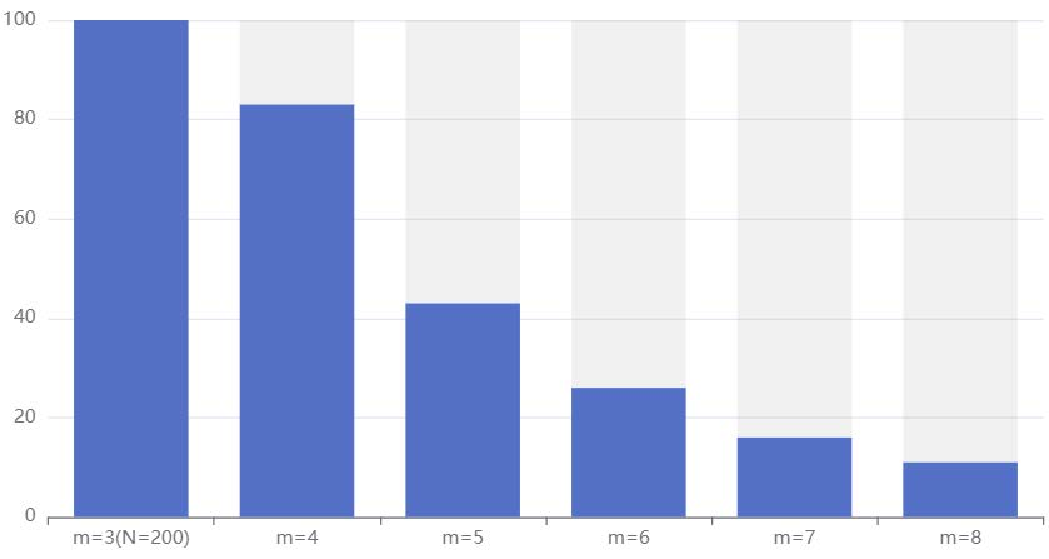
\includegraphics[width=0.8\textwidth]{nm_pairs.pdf}
    \caption{(n,m) pairs, y axis value represents n. For instance, when m=3, we test the pairs from $(n=1,m=3)$ to $(n=100,m=3)$, the second bar means we testing from $(n=1,m=4)$ to $(n=83,m=4)$}
\end{figure}\\
Figure 2 shows the accuracy test results for normal approximation(NA). The x axis is n and different colors represent different m values. As n increasing, MAE decreases for the same m value. We should also consider the effect of sparsity. As $n$ and $m$ raise, there will be a boost of number of probability mass points. Hence every probability mass point will be given less value averagely. Therefore, no matter what approximation method we apply here, the MAE will decrease as the number of probability mass points grows.

\begin{figure}%[h!]
    \centering
    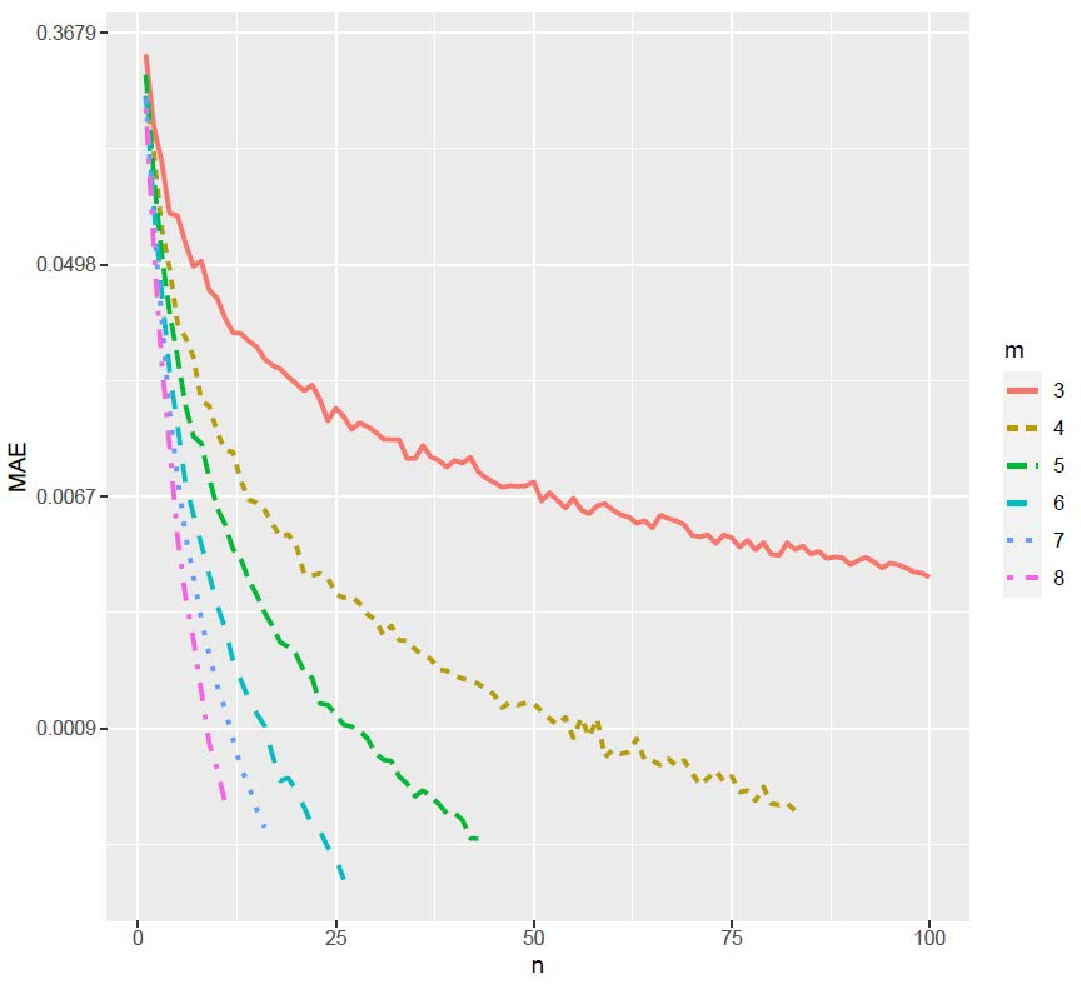
\includegraphics[width=0.8\textwidth]{normal_accuracy.pdf}
    \caption{Different colors and types of lines representing different $m$. The TAE is under log transformation}
\end{figure}


\subsubsection{Accuracy of Simulation Method}
While NA and MD-DFT can cover most cases, we introduce an other method for approximating PMDs', the simulation approximation method(SA). The idea behind this method is simple, as we know a PMD is a generalized multinomial distribution. Suppose each row of PMD matrix is a probability vector of a multinomial distribution, thus a $n\times m$ PMD matrix can be seen as n multinomial distributions with respect to n m-category probability vectors. Then we can have the following algorithm to approximate each probability mass point of PMD.

\begin{algorithm}%[H]
\SetAlgoLined
\KwResult{Write here the result }
 Set the repeating time equals to $N$\;
 \For{$t=1$ \KwTo $N$}{
  \For{$i=1$ \KwTo $n$}{
    generate 1 multinomial sample wrt probability vector = $i^{th}$ row of $P_{n \times m}$
  }
  sum up all samples generated in last loop and record the result as the $t^{th}$ row of matrix R.
 }
 \begin{itemize}
     \item compute the frequency of every result that stored in R as our probability mass point value.\\
     \item compare density calculated above and computed by MD-DFT to get MAE and TAE.
 \end{itemize}
 \caption{Simulation approximation algorithm (SA)}
\end{algorithm}

We also calculated the error bound of the simulation method.
Suppose for $i$th repeat, we consider random variable matrix $[X_{1i},X_{2i},\dots,X_{n i}]'$, each $X$ is a vector of length $m$ representing a voter's voting result. We repeat $R$ times to simulate the voting process to get $X_{j1},\dots,X_{j R}$ for each $j=1,\dots, n$, then
\begin{align*}
        &U_1 = \frac{\sum_{i=1}^{R} X_{1i}}{R} \longrightarrow N\left(p_1,\frac{1}{R}\left(Diag(p_1) - p_1 p_1'\right)\right)\\
        &U_2 = \frac{\sum_{i=1}^{R} X_{2i}}{R} \longrightarrow N\left(p_2,\frac{1}{R}\left(Diag(p_2) - p_2 p_2'\right)\right)\\
        & \vdots\\
        &U_n = \frac{\sum_{i=1}^{R} X_{ni}}{R} \longrightarrow N\left(p_n,\frac{1}{R}\left(Diag(p_n) - p_n p_n'\right)\right)
\end{align*}
Therefore
\begin{align*}
    U_1 + \dots + U_n \longrightarrow N\left(\sum_{i=1}^{n}p_i, \frac{1}{R}\sum_{i=1}^{n}\left(Diag(p_i) - p_i p_i'\right) \right)
\end{align*}
For each element in the vector $p_i$, say $p_{ij}$\\
\begin{equation*}
    p_{ij} - p_{ij}^2 \leq \frac{1}{4}
\end{equation*}
So the error of simulation will be controlled within
\begin{equation*}
    \frac{1}{R} \times \frac{n}{4} = \frac{n}{4R}
\end{equation*}

\begin{figure}%[h!]
    \centering
    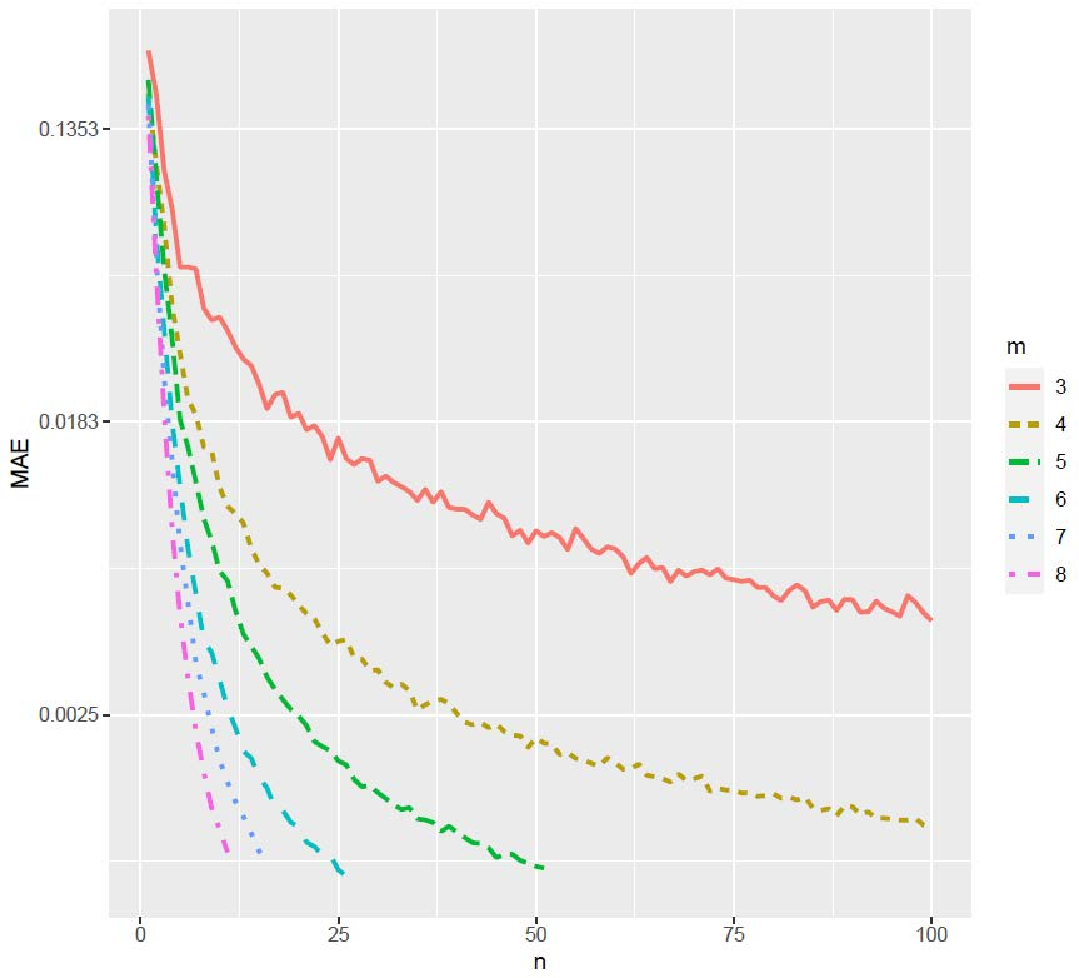
\includegraphics[width=0.8\textwidth]{simu_accuracy.pdf}
    \caption{Simulation accuracy test result, the repeating time set as $10^4$}
\end{figure}

Figure 3 illustrates the performance of SA method. For a fixed m and t, as n increases MAE decreases. Due to sparsity effect if we fix $n$, we could find MAE also drops while m increasing.

%%%%%%%%%%%%%%%%%%%%%%%%%%%%%%%%%%%%%%%%%%%%%%%%%%%%%%%%%%%%%%%%%%%%%%%%%%%%%%%%%%%%%%%%%%%%%%%%%
\subsection{Time Efficiency}
In this section, we show computation efficiency of simulation method and MD-DFT for calculating all probability mass points as $(n,m)$ gets large. We generate random matrices with respect to given $(n, m)$, record the calculating time of each method. As for normal approach, it is a asymptotic method, we only need to calculate the asymptotic normal distribution.

\begin{table}%[h!]
\centering
\caption{Accuracy of simulation method.}\label{tab:my_label}
\begin{tabular}{c|c|c}
\hline
\hline
     $(n, m)$ & MD-DFT & Simulation based $(10^6)$  \\
\hline
    (4, 3) & 0.023 & 0.542 \\
\hline
    (6, 3) & 0.002 & 0.852\\
\hline
    (8, 3) & 0.003 & 1.177\\
    (10, 3) & 0.003 & 1.634\\
    (20, 3) & 0.014 & 4.532\\
    (50, 3) & 0.098 & 22.349\\
    (100, 3) & 0.49 & 80.243\\
    (200, 3) & 2.834 & 307.350\\
    (1000, 3) & 249.449  & 7992.507 \\
\hline\hline
\end{tabular}
\end{table}
%%%%%%%%%%%%%%%%%%%%%%%%%%%%%%%%%%%%%%%%%%%%%%%%%%%%%%%%%%%%%%%%%%%%%%%%%%%%%%%%%%%%%%%%%%%%%%%%%
Study the computing of the three methods.


%%%%%%%%%%%%%%%%%%%%%%%%%%%%%%%%%%%%%%%%%%%%%%%%%%%%%%%%%%%%%%%%%%%%%%%%%%%%%%%%%%%%%%%%%%%%%%%%%
\subsection{Recommendations}
%%%%%%%%%%%%%%%%%%%%%%%%%%%%%%%%%%%%%%%%%%%%%%%%%%%%%%%%%%%%%%%%%%%%%%%%%%%%%%%%%%%%%%%%%%%%%%%%%

For small $m$ and moderate $n$, the MD-DFT can be used.

For large $m$ and moderate $n$, the simulation-based method can be used.

For large $n$, the NA-based method can be used.

%%%%%%%%%%%%%%%%%%%%%%%%%%%%%%%%%%%%%%%%%%%%%%%%%%%%%%%%%%%%%%%%%%%%%%%%%%%%%%%%%%%%%%
\section{Applications}
%%%%%%%%%%%%%%%%%%%%%%%%%%%%%%%%%%%%%%%%%%%%%%%%%%%%%%%%%%%%%%%%%%%%%%%%%%%%%%%%%%%%%%
\subsection{Calculation of Voting Probability}


Do some example like this:

https://stats.stackexchange.com/questions/274211/calculating-the-probability-of-someone-winning-from-a-poll




%%%%%%%%%%%%%%%%%%%%%%%%%%%%%%%%%%%%%%%%%%%%%%%%%%%%%%%%%%%%%%%%%%%%%%%%%%%%%%%%%%%%%%
\subsection{Statistical Inference for Aggregated Data}\label{sec:model.est.inf}	

Ecological inference

Examples of Using PMD in Heart Disease Data

Here we illustrate how to apply PMD in real data analysis by using hear disease data from UCI machine learning repository. The data was collected from multiple locations and here we only use the data from Cleveland.


The data contains 14 variables and 297 observations after removal of missing values, our response variable is the diagnosis of heart disease, it has 5 levels coded with 0, 1, 2, 3, 4. There are other 13 variables such as age, sex, exang(exercise induced angina) etc. In order to apply our methods of calculating PMD, we first divided the data into 61 smaller groups by 5 variables(chest pain type, sex, exercise induced angina, resting electrocardiographic results and the slope of the peak exercise ST segment), reader can also divide the data in other reasoning. We use 5 variables as our covariates as shown in the following table. Among the groups, $n$ varies from 2 to 62, which are affordable for MD-DFT method. A group of data is shown in Table 7.

\begin{table}%[h!]
    \centering
\begin{tabular}{|c|c|c|c|c|c|}

\hline
     age & trestbps & chol & thalach & oldpeak\\
\hline
      69 &  140 & 239  &  151  & 1.8\\
\hline
    60  & 150 & 24 & 171 & 0.9\\
\hline
\end{tabular}
    \caption{Selected Group of Heart Disease Data from Cleveland}
    \label{tab:my_label}
\end{table}

The total number for each level of our response variable in each group is known. WWe have 5 levels of response refer to 5 categories. In the example group shown in Table 7, the outcome vector is $\left(2,0,0,0,0\right)$ because both observations has response of level 0.

The first step is to estimate $P$ matrix for each group. Suppose the likelihood of each group is $\ell_1 ,\dots, \ell_{61}$, where $\ell_i = \text{the probability of getting the result of group i}$. We use softmax function to find 61 $P_i$ matrices for each one of the 61 groups. Then we can calculate $\ell_i$ via $P_i$, details are following.


Initiate values for parameters $\betavec = \left[\betavec_1,\dots,\betavec_5 \right]'$, where $\betavec_i = \left[\beta_{i1},\dots,\beta_{i5} \right]$ for our 5 categories and 5 covariates. Suppose we have $n_i$ observations in group $i$, the respecting $P_i$ matrix should be of dimension $n_i \times 5$, $P_i = \left(p_{jk}^{(i)}\right), j=1,\dots, n_i, k = 1, 2, 3, 4, 5$. Our observations are $X_i$, $i= 1, \dots, n_i$, each $X_i = \left[x_{i1},x_{i2},\dots, x_{i5}\right]$, where $x_{i1}, \dots, x_{i5}$ representing the covariates information.


Then we have the following $P_i$ matrix for each i by using softmax function,
\begin{align*}
    p_{jk}^{(i)} = \frac{\exp(\betavec'_{k}X_j)}{\sum_{h=1}^{5}\exp(\betavec'_{h}X_j)}
\end{align*}
After we get our $P_i$ matrices, apply MD-DFT or simulation or normal method, we get our likelihoods $\ell_i$ for $i = 1,\dots, 61$.


The total likelihood 
\begin{align}
L = \prod_{i=1}^{61}\ell_i.  
\end{align}
we can use numerical methods e.g., gradient descent, Newton method to find the $\betavec$ that maximized $L$, then we get our final $P_i$ matrices.\\


There are 3 categories and 2 observations, thus the $P$ matrix is $2 \times 3$. We calculate the $P$ matrix by using softmax function. The weights should be $4 \times 5$ dimension if we set the last category as baseline. By using MD-DFT we get the likelihood for the group getting result $\left(2,0,0\right)$. As we have 61 groups, we will have 61 likelihoods $l_1,\dots,l_{61}$ so that we can get a total likelihood $L = \prod_{i=1}^{61}l_i$.


We estimated the 61 $P$ matrices of 61 groups by maximizing $L$. Two of the P matrices are
\begin{align*}
    &P_1 =  \left[ \begin{array}{ccccc}
0.29725 &0.23646 &0.236462 &0.236462 &0.00058
 \\ 0.29749 & 0.23401& 0.23401& 0.23401 & 0.00047
 \end{array} \right]\\
\\
&P_{61} = \left[ \begin{array}{ccccc}
   0.28968 &  0.23646 &  0.23646 & 0.23646 & 0.00093
  \\
    0.31585 & 0.22798 & 0.22798 & 0.22798 & 0.00021
 \\
     0.29853 & 0.23343 & 0.23343 & 0.23343 & 0.00119
 \\
     0.30647 & 0.23093 & 0.23093 &  0.23093 &  0.00075
\end{array} \right]
\end{align*}
Therefore we hereby using our MD-DFT method again to calculate $P(X_1=2,X_2=0, X_3=0, X_4 = 0, X_5 = 0) =   0.08842$ and $P(X_1=0,X_2=1,X_3=2, X_4 - 1, X_5 = 0)=0.03487$


%%%%%%%%%%%%%%%%%%%%%%%%%%%%%%%%%%%%%%%%%%%%%%%%%%%%%%%%%%%%%%%%%%%%%%%%%%%%%%%%%%%%%%
\subsection{Uncertainty Quantification in Classification}

Confusion matrix

Use Theorem for independent.

In machine learning classification problem with multiple labels, for each unit in the test set, the probability of the unit belongs to each class is computed. Usually, the predicted class is assigned as the highest probability. In the classifiers (i.e., soft classification), the unit class is randomly assigned according to the predicted probabilities, leading to randomness in the confusion matrix. The PMD can be used to characterize the distribution of the counts in the confusion matrix. 



Yueyao: reliability course project used EL images for classification. The confusion matrix is obtained (Table 4 of the course report). In some senses, Table 4 only provide the point estimates, with PMD the distribution of the counts in each cell can be found, and can be displayed by an array of histograms. 




%%%%%%%%%%%%%%%%%%%%%%%%%%%%%%%%%%%%
\section{Illustrations of the R Package}
%%%%%%%%%%%%%%%%%%%%%%%%%%%%%%%%%%%%%%%%%%%%%%%%%%%%%%%%%%%%%%%%%%%%%%%%%%%%%%%%%%%%%%%%%%%%%%%%%
\subsection{Examples}
Illustrate the use of major functions in the R package.


%%%%%%%%%%%%%%%%%%%%%%%%%%%%%%%%%%%%%%%%%%%%%%%%%%%%%%%%%%%%%%%%%%%%%%%%%%%%%%%%%%%%%%%%%%%%%%%%%
\subsection{Benchmark of R Packages for Poisson Binomial Distribution}
%%%%%%%%%%%%%%%%%%%%%%%%%%%%%%%%%%%%%%%%%%%%%%%%%%%%%%%%%%%%%%%%%%%%%%%%%%%%%%%%%%%%%%%%%%%%%%%%%



%%%%%%%%%%%%%%%%%%%%%%%%%%%%%%%%%%%%%%%%%%%%%%%%%%%%%%%%%%%%%%%%%%%%%%%%%%%%%%%%%%%%%%%%%%%%%%%%%
\section{Conclusions and Areas for Future Research}
%%%%%%%%%%%%%%%%%%%%%%%%%%%%%%%%%%%%%%%%%%%%%%%%%%%%%%%%%%%%%%%%%%%%%%%%%%%%%%%%%%%%%%%%%%%%%%%%%

We develop algorithm that can be useful for computing the pmf of the PMD distribution, which is challenging to compute but useful in many application scenarios.





	
%%%%%%%%%%%%%%%%%%%%%%%%%%%%%%%%%%%%%%%%%%%%%%%%%%%%%%%%%%%%%%%%%%%%%%%%%%%%%%%%%%%%%%%%%%%%%%%%%%%%%%%%%%%%%%%%%%%%

%\section*{Acknowledgments}
%%%%%%%%%%%%%%%%%%%%%%%%%%%%%%%%%%%%%%%%%%%%%%%%%%%%%%%%%%%%%%%%%%%%%%%%%%%%%%%%%%%%%%%%%%%%%%%%%%%%%%%%%%%%%%%%%

%\bibliographystyle{apacite}


\bibliographystyle{chicago}
\bibliography{refs}	

\end{document}

%%%%%%%%%%%%%%%%%%%%%%%%%%%%%%%%%%%%%%%%%%%%%%%%%%%%%%%%%%%%%%%%%%%%%%%%%%%%%%%%%%%%%%%%%%%%%%%%%%%%%%%%%%%%%%%%%%%%%%%%%%%%%%%%%%%%%%%

